% ==================================================================
% 3.1 Detector platform.
% Hinh fig3_arch GANH phan mo ta kien truc -> van o day co y giu NGAN:
% chi noi cai gi hinh khong noi duoc (ly do thiet ke + con so chi phi).
% Kien truc KHONG phai dong gop cua bai (Section 4.4 noi thang the).
% file: sections/05_platform.tex
% ==================================================================
\subsection{Detector Platform}
\label{sec:platform}

\begin{figure}[t]
\centering
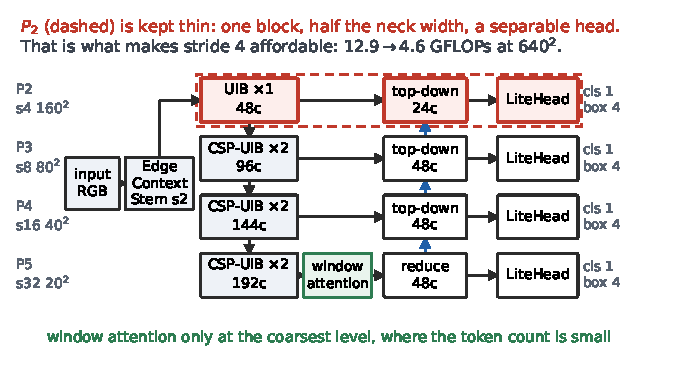
\includegraphics[width=0.95\textwidth]{figures/fig3_arch.pdf}
\caption{SteadyDet-N; resolution decreases down the page. Compute is deliberately
asymmetric: the stride-4 row $P_2$ (dashed), where most drone-scale persons are
resolved, carries one block, a half-width neck branch and a separable head, while
the two-block CSP stages and the attention sit where the maps are small. Blue
arrows are the top-down upsample-and-fuse path. That is what keeps $P_2$ at $4.6$
instead of $12.9$ GFLOPs.}
\label{fig:arch}
\end{figure}

SteadyDet-N is an anchor-free single-stage detector of $1.17$\,M parameters and
$4.6$ GFLOPs at $640\times640$ (Fig.~\ref{fig:arch}). We are explicit about what we
do and do not claim for it. It does not lead its class in clean accuracy and
Section~\ref{sec:baselines} reports that plainly; what we claim is its accuracy
under vibration once the corruption is in its training distribution, a combination
no baseline we measured matches. The design choice that matters most for this is
that it keeps a stride-4 level, since at the altitudes VisDrone covers a person
occupies fewer than $32\times32$ pixels and detectors beginning at stride 8 discard
that signal before detection begins.

Keeping stride 4 is what makes such a detector expensive. At $640\times640$ the $P_2$
map is $160\times160$, so every operation there costs $16\times$ what it costs at
$P_3$, and in an earlier configuration of ours the $P_2$ head alone consumed $1.82$
GMACs, $28\%$ of total compute. Fig.~\ref{fig:arch} shows the three changes that cut
the total to $4.6$ GFLOPs without giving up stride 4: one Universal Inverted
Bottleneck~\cite{qin2024mnv4} block at $P_2$ instead of three, windowed
self-attention~\cite{liu2021swin} at $P_5$ only, and a depthwise-separable head in
place of a five-convolution decoupled one. Deeper stages use cross-stage partial
blocks~\cite{wang2020cspnet}.

Regression blends the Normalized Wasserstein Distance~\cite{wang2021nwd} with
CIoU~\cite{zheng2020diou} by ground-truth area, since IoU gradients are unstable for
tiny boxes; classification uses~\cite{li2020gfl} and assignment
follows~\cite{feng2021tood}, modified so each small ground truth gets several
positives. Optimisation blends Muon~\cite{jordan2024muon} and SGD.
